\pdfminorversion=7
\documentclass[aspectratio=169,10pt]{beamer}

\usepackage[utf8]{inputenc}
\usepackage[T1]{fontenc}
\usepackage[italian]{babel}
\usepackage{lmodern}
\usepackage{graphicx}
\usepackage{tikz}
\usetikzlibrary{arrows.meta,positioning,shapes.geometric}

\graphicspath{{../images/}}

\definecolor{UnibsBlue}{HTML}{0B3C5D}
\definecolor{AccentTeal}{HTML}{1F7A8C}
\definecolor{AccentGold}{HTML}{C88A1A}
\definecolor{AccentRed}{HTML}{B2483E}
\definecolor{SoftBg}{HTML}{F4F7F9}
\definecolor{SoftLine}{HTML}{D7E0E7}
\definecolor{SoftText}{HTML}{425466}

\setbeamertemplate{navigation symbols}{}
\setbeamertemplate{itemize item}{\color{UnibsBlue}\small$\blacksquare$}
\setbeamercolor{normal text}{fg=black,bg=white}
\setbeamercolor{frametitle}{fg=UnibsBlue}
\setbeamercolor{title}{fg=UnibsBlue}
\setbeamercolor{structure}{fg=UnibsBlue}
\setbeamerfont{title}{size=\LARGE,series=\bfseries}
\setbeamerfont{frametitle}{size=\large,series=\bfseries}
\setbeamerfont{footline}{size=\scriptsize}

\setbeamertemplate{footline}{%
  \leavevmode%
  \hbox{%
    \begin{beamercolorbox}[wd=\paperwidth,ht=2.8ex,dp=1.2ex,right]{footline}%
      \color{SoftText}\insertframenumber/\inserttotalframenumber\hspace*{1em}
    \end{beamercolorbox}%
  }%
}

\newcommand{\tagitem}[1]{%
  \tikz[baseline=(node.base)] \node[
    rounded corners=4pt,
    fill=SoftBg,
    draw=SoftLine,
    inner xsep=6pt,
    inner ysep=3pt,
    text=UnibsBlue,
    font=\scriptsize\bfseries
  ] (node) {#1};%
}

\newcommand{\techbox}[4]{%
  \begin{tikzpicture}
    \node[
      rounded corners=10pt,
      draw=SoftLine,
      fill=SoftBg,
      minimum width=3.45cm,
      minimum height=4.2cm,
      align=center
    ] (box) {};
    \node[font=\bfseries\large,text=UnibsBlue] at (0,1.2) {#1};
    \node[
      circle,
      fill=white,
      draw=AccentTeal,
      line width=1pt,
      minimum size=0.9cm,
      font=\bfseries\small,
      text=AccentTeal
    ] at (0,0.25) {#2};
    \node[font=\scriptsize\bfseries,text=AccentTeal] at (0,-0.55) {#3};
    \node[font=\scriptsize\bfseries,text=AccentRed] at (0,-1.15) {#4};
  \end{tikzpicture}
}

\title{SafeSwitch, 5G e platooning sicuro}
\subtitle{Valutazione simulativa di un protocollo 5G-V2X per lo smantellamento sicuro di platoon}
\author{Alex Marchi}
\date{A.A. 2025/2026}

\begin{document}

\begin{frame}[plain]
  \begin{columns}[T,totalwidth=\textwidth]
    \column{0.60\textwidth}
      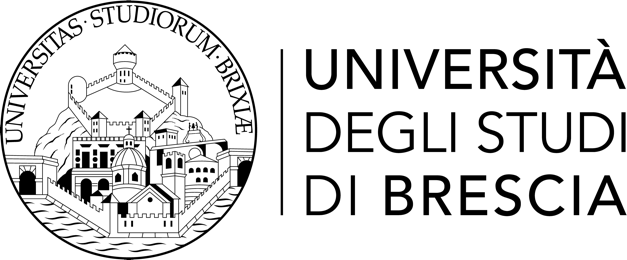
\includegraphics[width=0.28\linewidth]{logo_unibs.png}

      \vspace{0.8em}
      {\usebeamerfont{title}\color{UnibsBlue}SafeSwitch, 5G\\e platooning sicuro\par}
      \vspace{0.4em}
      {\small\color{SoftText}Valutazione simulativa di un protocollo 5G-V2X\\per lo smantellamento sicuro di platoon\par}

      \vspace{1em}
      \tagitem{Platooning}\hspace{0.4em}
      \tagitem{SafeSwitch}\hspace{0.4em}
      \tagitem{Simu5G}

      \vspace{1.3em}
      {\small\color{SoftText}
      Obiettivo: verificare che \textit{SafeSwitch} resti valido\\
      in una toolchain aggiornata e con 5G al posto di LTE.}

    \column{0.36\textwidth}
      \begin{beamercolorbox}[
        rounded=true,
        sep=1em,
        shadow=false,
        wd=\linewidth
      ]{}
        \color{UnibsBlue}\textbf{Alex Marchi}

        \vspace{0.6em}
        \color{SoftText}\small
        Laurea in Ingegneria Informatica

        \vspace{0.8em}
        Relatori\\
        Prof. Renato Lo Cigno\\
        Dott. Lorenzo Ghiro

        \vspace{0.8em}
        Matricola 727612
      \end{beamercolorbox}
  \end{columns}
\end{frame}

\begin{frame}{Il problema}
  \begin{columns}[T,totalwidth=\textwidth]
    \column{0.50\textwidth}
      \centering
      \resizebox{\linewidth}{!}{%
      \begin{tikzpicture}[x=1cm,y=1cm]
        \foreach \x/\label in {0/Leader,2.2/Follower,4.4/Follower,6.6/Follower} {
          \draw[rounded corners=2pt,fill=SoftBg,draw=UnibsBlue,thick] (\x,0.2) rectangle +(1.6,0.7);
          \draw[fill=black] (\x+0.25,0.15) circle (0.08);
          \draw[fill=black] (\x+1.35,0.15) circle (0.08);
          \node[font=\scriptsize\bfseries,text=UnibsBlue] at (\x+0.8,1.25) {\label};
        }
        \foreach \x in {1.65,3.85,6.05} {
          \draw[-{Latex[length=3mm]},AccentTeal,thick] (\x,0.95) -- +(0.55,0);
          \node[font=\tiny\bfseries,text=AccentTeal] at (\x+0.28,1.2) {V2X};
        }
        \foreach \x in {1.60,3.80,6.00} {
          \draw[SoftLine,thick] (\x,0.55) -- +(0.6,0);
          \node[font=\tiny,text=SoftText] at (\x+0.3,0.25) {gap ridotto};
        }
      \end{tikzpicture}%
      }

      \vspace{0.8em}
      {\small\color{SoftText}Il vantaggio del platooning nasce da veicoli vicini\\
      e coordinati in tempo reale.}

    \column{0.46\textwidth}
      \begin{beamercolorbox}[rounded=true,sep=0.8em,wd=\linewidth]{}
        \textbf{\color{UnibsBlue}Benefici}

        \small\color{SoftText}
        più capacità stradale\\
        meno consumi\\
        guida più regolare
      \end{beamercolorbox}

      \vspace{0.8em}
      \begin{beamercolorbox}[rounded=true,sep=0.8em,wd=\linewidth]{}
        \textbf{\color{AccentRed}Criticità}

        \small\color{SoftText}
        se la comunicazione peggiora, peggiora anche il controllo
      \end{beamercolorbox}

      \vspace{0.8em}
      \begin{beamercolorbox}[rounded=true,sep=0.8em,wd=\linewidth]{}
        \textbf{\color{AccentGold}Domanda della tesi}

        \small\color{SoftText}
        come mantenere il platoon sicuro quando il link degrada?
      \end{beamercolorbox}
  \end{columns}
\end{frame}

\begin{frame}{Tre interfacce, tre guasti diversi}
  \centering
  \techbox{802.11p}{R}{diretto}{contesa / interferenza}
  \hspace{0.35cm}
  \techbox{VLC}{L}{preciso}{linea di vista}
  \hspace{0.35cm}
  \techbox{5G}{C}{copertura}{handover}

  \vspace{1.2em}
  \begin{beamercolorbox}[rounded=true,sep=0.9em,wd=0.85\linewidth]{}
    \centering
    \textbf{\color{UnibsBlue}Idea chiave}

    \vspace{0.3em}
    \small\color{SoftText}
    i beacon vengono inviati in parallelo sulle interfacce attive,\\
    così il sistema sfrutta \textbf{ridondanza} e \textbf{complementarità}
  \end{beamercolorbox}
\end{frame}

\begin{frame}{Come funziona SafeSwitch}
  \begin{columns}[T,totalwidth=\textwidth]
    \column{0.52\textwidth}
      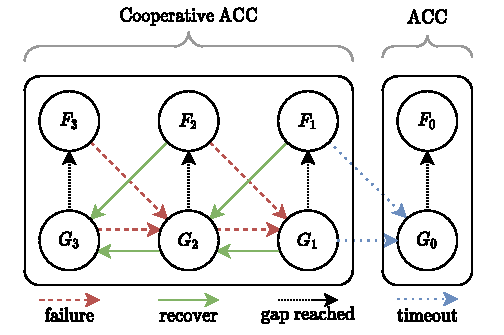
\includegraphics[width=\linewidth]{fallback-fsm.pdf}

    \column{0.44\textwidth}
      \begin{beamercolorbox}[rounded=true,sep=0.8em,wd=\linewidth]{}
        \textbf{\color{UnibsBlue}1. Monitoraggio}

        \small\color{SoftText}
        PDR su leader e predecessore
      \end{beamercolorbox}

      \vspace{0.45em}
      \centering{\Large\color{SoftText}$\Downarrow$}

      \begin{beamercolorbox}[rounded=true,sep=0.8em,wd=\linewidth]{}
        \textbf{\color{UnibsBlue}2. Failure / recovery}

        \small\color{SoftText}
        ogni follower decide localmente
      \end{beamercolorbox}

      \vspace{0.45em}
      \centering{\Large\color{SoftText}$\Downarrow$}

      \begin{beamercolorbox}[rounded=true,sep=0.8em,wd=\linewidth]{}
        \textbf{\color{UnibsBlue}3. Gap control}

        \small\color{SoftText}
        prima adatto la distanza, poi cambio controllore
      \end{beamercolorbox}

      \vspace{0.8em}
      \begin{beamercolorbox}[rounded=true,sep=0.7em,wd=\linewidth]{}
        \centering
        \textbf{\color{AccentRed}Niente switch bruschi da CACC ad ACC}
      \end{beamercolorbox}
  \end{columns}
\end{frame}

\begin{frame}{Il mio contributo}
  \centering
  \begin{tikzpicture}[node distance=1.15cm]
    \node[
      rounded corners=10pt,
      draw=SoftLine,
      fill=SoftBg,
      minimum width=3.55cm,
      minimum height=2.7cm,
      align=center
    ] (a) {
      \textbf{\color{UnibsBlue}Ricostruzione stack}\\[0.4em]
      \small\color{SoftText}
      OMNeT++\\Veins\\PLEXE\\SUMO
    };
    \node[
      rounded corners=10pt,
      draw=SoftLine,
      fill=SoftBg,
      minimum width=3.55cm,
      minimum height=2.7cm,
      align=center,
      right=1.3cm of a
    ] (b) {
      \textbf{\color{UnibsBlue}Porting di SafeSwitch}\\[0.4em]
      \small\color{SoftText}
      PDR\\FSM\\scenari\\metriche
    };
    \node[
      rounded corners=10pt,
      draw=SoftLine,
      fill=SoftBg,
      minimum width=3.55cm,
      minimum height=2.7cm,
      align=center,
      right=1.3cm of b
    ] (c) {
      \textbf{\color{UnibsBlue}Migrazione LTE $\rightarrow$ 5G}\\[0.4em]
      \small\color{SoftText}
      SimuLTE out\\Simu5G in\\\texttt{plexe\_hetnet}
    };

    \draw[-{Latex[length=4mm]},thick,AccentTeal] (a) -- (b);
    \draw[-{Latex[length=4mm]},thick,AccentTeal] (b) -- (c);
  \end{tikzpicture}

  \vspace{1.1em}
  \begin{beamercolorbox}[rounded=true,sep=0.9em,wd=0.9\linewidth]{}
    \centering
    \textbf{\color{AccentGold}Messaggio chiave}

    \vspace{0.3em}
    \small\color{SoftText}
    ho mantenuto \textbf{la stessa logica multi-interfaccia} del lavoro originale,\\
    aggiornando però \textbf{la componente cellulare} e la \textbf{toolchain}
  \end{beamercolorbox}
\end{frame}

\begin{frame}{Risultato 1: SafeSwitch serve davvero}
  \centering
  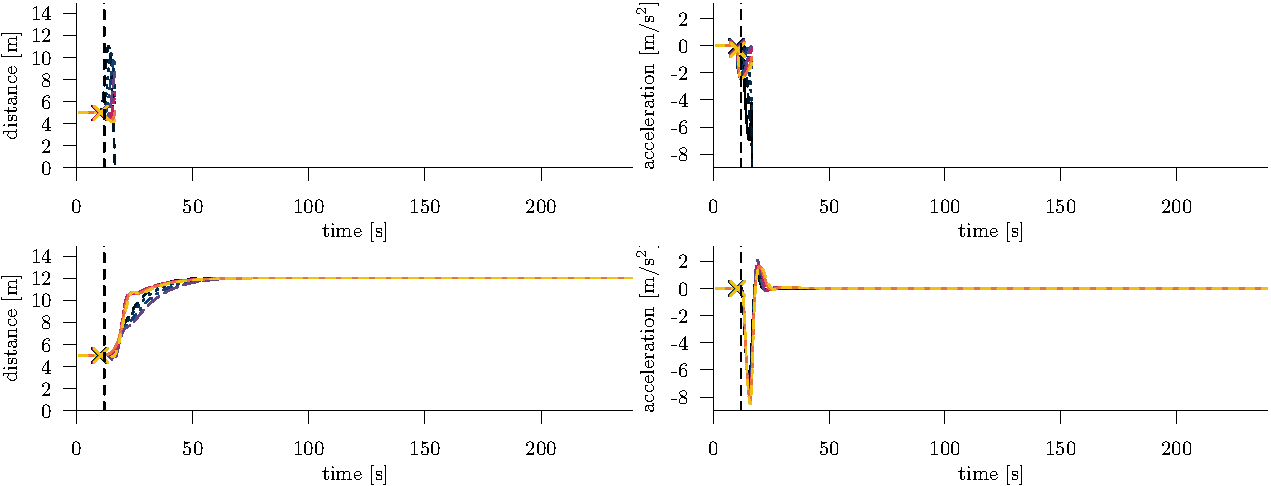
\includegraphics[width=\linewidth,height=0.68\textheight,keepaspectratio]{scenario_3-grid.pdf}

  \vspace{0.3em}
  \begin{columns}[T,totalwidth=\textwidth]
    \column{0.48\textwidth}
      \begin{beamercolorbox}[rounded=true,sep=0.7em,wd=\linewidth]{}
        \centering
        \textbf{\color{AccentRed}Fallback naive}

        \small\color{SoftText}
        switch diretto\\collisione
      \end{beamercolorbox}
    \column{0.48\textwidth}
      \begin{beamercolorbox}[rounded=true,sep=0.7em,wd=\linewidth]{}
        \centering
        \textbf{\color{AccentTeal}SafeSwitch}

        \small\color{SoftText}
        transizione graduale\\platoon salvo
      \end{beamercolorbox}
  \end{columns}
\end{frame}

\begin{frame}{Risultato 2: il 5G preserva il comportamento}
  \centering
  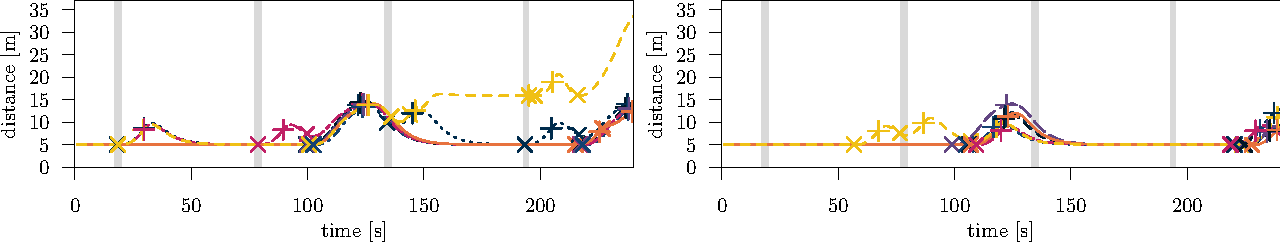
\includegraphics[width=\linewidth,height=0.66\textheight,keepaspectratio]{distance-side-by-side.pdf}

  \vspace{0.15em}
  {\small\color{SoftText}sinistra: articolo di riferimento \hspace{1.5em} destra: risultati della tesi\par}

  \vspace{0.35em}
  \begin{columns}[T,totalwidth=\textwidth]
    \column{0.31\textwidth}
      \begin{beamercolorbox}[rounded=true,sep=0.65em,wd=\linewidth]{}
        \centering
        \small\textbf{\color{UnibsBlue}stessa dinamica qualitativa}
      \end{beamercolorbox}
    \column{0.31\textwidth}
      \begin{beamercolorbox}[rounded=true,sep=0.65em,wd=\linewidth]{}
        \centering
        \small\textbf{\color{UnibsBlue}picchi più contenuti}
      \end{beamercolorbox}
    \column{0.31\textwidth}
      \begin{beamercolorbox}[rounded=true,sep=0.65em,wd=\linewidth]{}
        \centering
        \small\textbf{\color{UnibsBlue}handover meno severi}
      \end{beamercolorbox}
  \end{columns}
\end{frame}

\begin{frame}{Conclusioni}
  \begin{beamercolorbox}[rounded=true,sep=1em,wd=\linewidth]{}
    \centering
    \Large\textbf{\color{UnibsBlue}SafeSwitch resta coerente anche in uno stack aggiornato con 5G}
  \end{beamercolorbox}

  \vspace{1em}
  \begin{columns}[T,totalwidth=\textwidth]
    \column{0.48\textwidth}
      \begin{beamercolorbox}[rounded=true,sep=0.9em,wd=\linewidth]{}
        \textbf{\color{UnibsBlue}Perché conta}

        \small\color{SoftText}
        rete, controllo e sicurezza vanno progettati insieme\\[0.3em]
        il 5G rende l'ambiente più attuale\\[0.3em]
        il lavoro diventa una base riusabile
      \end{beamercolorbox}

    \column{0.48\textwidth}
      \begin{beamercolorbox}[rounded=true,sep=0.9em,wd=\linewidth]{}
        \textbf{\color{UnibsBlue}Sviluppi futuri}

        \small\color{SoftText}
        scenari più realistici e canali più ricchi\\[0.3em]
        confronto LTE/5G più controllato\\[0.3em]
        veicoli e dotazioni eterogenee
      \end{beamercolorbox}
  \end{columns}

  \vspace{1em}
  \centering
  {\small\color{SoftText}In pratica: una base per studiare sistemi V2X che si degradano in modo sicuro.}
\end{frame}

\end{document}
